% Copyright 2004 by Till Tantau <tantau@users.sourceforge.net>.
%
% In principle, this file can be redistributed and/or modified under
% the terms of the GNU Public License, version 2.
%
% However, this file is supposed to be a template to be modified
% for your own needs. For this reason, if you use this file as a
% template and not specifically distribute it as part of a another
% package/program, I grant the extra permission to freely copy and
% modify this file as you see fit and even to delete this copyright
% notice. 

\documentclass{beamer}

\usepackage{fontspec} % Need this to use Optima
\setsansfont{Optima} % Set main font here

% There are many different themes available for Beamer. A comprehensive
% list with examples is given here:
% http://deic.uab.es/~iblanes/beamer_gallery/index_by_theme.html
% You can uncomment the themes below if you would like to use a different
% one:
%\usetheme{AnnArbor}
%\usetheme{Antibes}
%\usetheme{Bergen}
%\usetheme{Berkeley}
%\usetheme{Berlin}
%\usetheme{Boadilla}
%\usetheme{boxes}
%\usetheme{CambridgeUS}
%\usetheme{Copenhagen}
%\usetheme{Darmstadt}
%\usetheme{default}
%\usetheme{Frankfurt}
%\usetheme{Goettingen}
%\usetheme{Hannover}
%\usetheme{Ilmenau}
%\usetheme{JuanLesPins}
%\usetheme{Luebeck}
\usetheme{Madrid}
%\usetheme{Malmoe}
%\usetheme{Marburg}
%\usetheme{Montpellier}
%\usetheme{PaloAlto}
%\usetheme{Pittsburgh}
%\usetheme{Rochester}
%\usetheme{Singapore}
%\usetheme{Szeged}
%\usetheme{Warsaw}

\title{Uncovering Hidden Structure in the \textit{De Re Publica}}
\subtitle{A Computational Analysis of the Text}

% A subtitle is optional and this may be deleted
%\subtitle{Optional Subtitle}

\author{Marc E. Canby}
% - Give the names in the same order as the appear in the paper.
% - Use the \inst{?} command only if the authors have different
%   affiliation.

\institute[] % (optional, but mostly needed)
{
	\inst{}%
	Lati 318 $-$ Cicero: \textit{De Re Publica}\\
	Rice University

%	\inst{2}%
%	Department of Theoretical Philosophy\\
%	University of Elsewhere
}
% - Use the \inst command only if there are several affiliations.
% - Keep it simple, no one is interested in your street address.

\date{}
% - Either use conference name or its abbreviation.
% - Not really informative to the audience, more for people (including
%   yourself) who are reading the slides online

%\subject{Theoretical Computer Science}
% This is only inserted into the PDF information catalog. Can be left
% out. 

% If you have a file called "university-logo-filename.xxx", where xxx
% is a graphic format that can be processed by latex or pdflatex,
% resp., then you can add a logo as follows:

% \pgfdeclareimage[height=0.5cm]{university-logo}{university-logo-filename}
% \logo{\pgfuseimage{university-logo}}

% Delete this, if you do not want the table of contents to pop up at
% the beginning of each subsection:
\AtBeginSection[]
{
\begin{frame}<beamer>{Outline}
\tableofcontents
[
currentsection,
%currentsubsection,
%subsectionstyle=show
subsectionstyle=show/show/shaded
]
\end{frame}
}

% Change numbers in table of contents
\setbeamertemplate{section in toc}{\inserttocsectionnumber.~\inserttocsection}

% make symbols bold
\newcommand{\bld}[1]{\boldsymbol{#1}}

% for long division
\usepackage{array}
\usepackage{polynom}

% algorithms
\usepackage[]{algorithm2e}

\usepackage{tabto} % tabbing

% Change spacing in outline
\usepackage{etoolbox}
\makeatletter
\patchcmd{\beamer@sectionintoc}
{\vfill}
{\vskip\itemsep}
{}
{}
\makeatother  

% Arrows
\usepackage{tikz}
\usetikzlibrary{shapes.arrows}

\tikzset{
	myarrow/.style={
		draw,
		fill=blue,
		single arrow,
		minimum height=3ex,

		single arrow head extend=1ex
	}
}
\newcommand{\arrowdown}{%
	\tikz [baseline=-1ex]{\node [myarrow,rotate=-90] {};}
}

% Let's get started
\begin{document}

\begin{frame}
\titlepage
\end{frame}

\begin{frame}{Outline}
\tableofcontents
\end{frame}

\section{Getting and Cleaning the Data}

\begin{frame}{Getting and Cleaning the Data}


\begin{itemize}
	\setlength\itemsep{1em}
	\item Text obtained from \textit{The Latin Library} at the sentence level:
	\begin{itemize}
		\item {\ttfamily ['nempe',
		'ab',
		'iis',
		'qui',
		'haec',
		'disciplinis',
		'informata',
		'alia',
		'moribus',
		'confirmarunt',
		',',
		'sanxerunt',
		'autem',
		'alia',
		'legibus',
		'.']}
	\end{itemize}
\item Cleaned up messy elements of data:
\begin{itemize}
	\setlength\itemsep{0.5em}
	\item Line numbers: {\ttfamily [1,2,...,71]}
	\item Angle brackets: {\ttfamily ['\&',
		'lt',
		';',
		'im\&gt',
		';',
		'petu',
		'liberavissent',
		',',
		'nec',...]}
	\begin{itemize}
		\item {\ttfamily \&lt;} should be {\ttfamily <} \qquad {\ttfamily \&gt;} should be {\ttfamily >}
	\end{itemize}
\item Hyphens encoded as {\ttfamily \&\#}
\item English words: {\ttfamily ['Cicero', 'The', 'Latin', 'Library', 'The', 'Classics', 'Page']}
\end{itemize}
\end{itemize}

\end{frame}




\section{Exploratory Text Analysis}

\begin{frame}{Exploratory Text Analysis: Tokenization and POS Tagging}
\begin{itemize}
	\item Map each word to its base form (\textit{lemma} or \textit{token}) and its POS
	\item Often ignore \textit{stop words} ('et', 'sum', etc.) $-$ highlighted in red
\end{itemize}
\begin{center}
	{\ttfamily ['nempe',
		'ab',
		'iis',
		'qui',
		'haec',
		'disciplinis',
		'informata',
		'alia',
		'moribus',
		'confirmarunt',
		',',
		'sanxerunt',
		'autem',
		'alia',
		'legibus',
		'.']}\\
	
\begin{tikzpicture}
	\pgfsetarrowsend{latex}
	\pgfsetlinewidth{2ex}
	\pgfpathmoveto{\pgfpointorigin}
	\pgfpathlineto{\pgfpoint{3.5cm}{2cm}}
	\pgfusepath{stroke}
	\useasboundingbox (-02,-0.25) rectangle (0,0.5);
	\end{tikzpicture}
	
	{\ttfamily[('nempe', 'adverb'),
		{\color{red} ('ab', 'preposition')},
		{\color{red}('is', 'pronoun')},
		{\color{red}('qui', 'pronoun')},
		{\color{red}('hic', 'pronoun')},
		('disciplina', 'noun'),
		('informo', 'noun'),
		('alius2', 'adjective'),
		('mos', 'noun'),
		('confirmo', 'verb'),
		('sancio', 'verb'),
		{\color{red}('autem', 'conjunction')},
		('alius2', 'adjective'),
		('lex', 'noun')]}
	
\end{center}
\end{frame}

\begin{frame}{Exploratory Text Analysis}
\begin{itemize}
	\item Number of characters: 109,777 \tab (\textit{average:} 136,893)
	\item Number of words: 20,067 \tab (\textit{average:} 24,924)
	\item Number of sentences: 820 \tab (\textit{average:} 1,059)
\end{itemize}



\begin{figure}
	\centering
	\begin{minipage}{.5\textwidth}
		\centering
		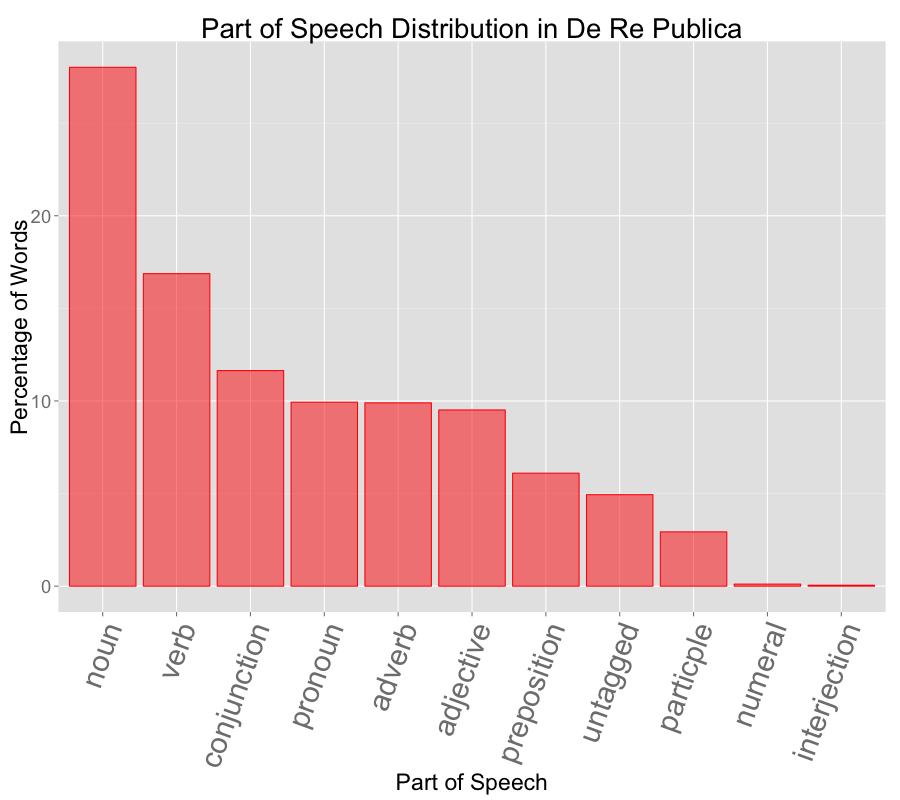
\includegraphics[scale=0.19]{fig1.png}
	\end{minipage}%
	\begin{minipage}{.5\textwidth}
		\centering
		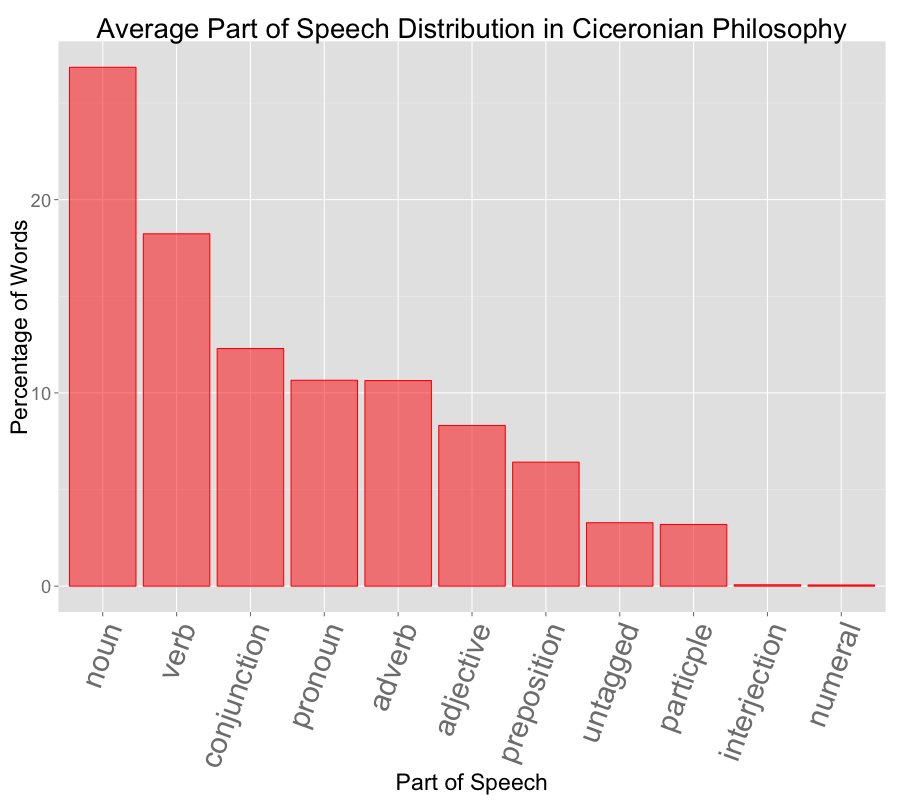
\includegraphics[scale=0.19]{fig2.png}
	\end{minipage}
\end{figure}
\end{frame}

\section{Underlying Word Structure: Word2Vec}



\end{document}


